
%-----------------------------------------------------------------------
%
% filename = usermanual.tex
% 
%-----------------------------------------------------------------------

\documentclass[12pt]{article}

% Load packages for symbols and figures.

\usepackage{latexsym}
\usepackage{epsfig}
\usepackage{amsmath}
\usepackage{amssymb}
\usepackage{tikz}
\usetikzlibrary{shapes}

% Page settings.

\setlength{\textwidth}{170mm}
\setlength{\oddsidemargin}{-5mm}
\setlength{\evensidemargin}{-5mm}


%%%%%%%%%%%%%%%%%%%%%%%%%%
%%%   BEGIN DOCUMENT   %%%
%%%%%%%%%%%%%%%%%%%%%%%%%%

\begin{document}

% Reference equations with section number.

\renewcommand{\theequation}{\thesection.\arabic{equation}}

\parindent 0mm


%%%%%%%%%%%%%%%%%
%%%   TITLE   %%%
%%%%%%%%%%%%%%%%%

\title{Code \texttt{OllinAxis-BiB} \\ User's manual}

\author{Miguel Alcubierre \\
Instituto de Ciencias Nucleares, UNAM \\
malcubi@nucleares.unam.mx}

\date{February, 2026}

\maketitle

\tableofcontents


%%%%%%%%%%%%%%%%%%%%%%%%
%%%   INTRODUCTION   %%%
%%%%%%%%%%%%%%%%%%%%%%%%

\pagebreak

\section{Introduction}

This program solves the Einstein evolution equations in axial symmetry
using a curvilinear version of the BSSN formulation for the 3+1
evolution equations, with different types of matter and different
gauge conditions. \\

The main difference of this version of the code with respect to
previous ones is the fact that it uses box-in-box mesh refinement
(hence the BiB part of the name), and is parallelized with MPI.
Many parts of this code are based on a previous version written
by myself and José Manuel Torres.  An even older version was
written by Milton Ruiz. \\

Note: THIS MANUAL IS STILL INCOMPLETE!  I haven't had the time to
finish it. Still, it should give you a good idea of the basics. I will
be adding a little bit more every now and again. \\


%%%%%%%%%%%%%%%%%%%%
%%%   DOWNLOAD   %%%
%%%%%%%%%%%%%%%%%%%%

\section{Downloading the code}

If you are reading this it means you probably already downloaded the
code.  But if for some reason you need to download it here is how. \\

The easiest way to obtain the code is to download it from GitHub: \\

\texttt{\footnotesize git clone https://github.com/malcubi/OllinAxis-BiB} \\

Once you have the code, you can get updated versions by just doing
``git pull'' inside the code main directory.


%%%%%%%%%%%%%%%%%%%%%%%
%%%   DIRECTORIES   %%%
%%%%%%%%%%%%%%%%%%%%%%%

\section{Directory structure}

The main directory for the code is \texttt{OllinAxis-BiB}.  There are
several sub-directories inside this main directory:

\begin{list}{}{
\setlength{\leftmargin}{40mm}
\setlength{\labelsep}{10mm}
\setlength{\labelwidth}{25mm}}

\item[\texttt{CVS}] Contains information about the CVS root and server (see
Sec.~\ref{sec:editing}).

\item[\texttt{doc}] Contains the tex and pdf files for this user's
  manual.

\item[\texttt{exe}] This directory is created at compile time and
  contains the executable file.  It also contains a copy of the
  parameter files found in directory \texttt{par} (see below).

\item[\texttt{fakempi}] Contains fake MPI routines so that the
  compiler won't complain if MPI is not installed.

\item[\texttt{gnuplot}] Contains a couple of simple gnuplot macros for
  visualization.

\item[\texttt{objs}] This directory is created at compile time and
  contains all the object and module files.

\item[\texttt{ollingraph}] Contains the visualization packages
  ``ollingraph'' and ``ollingraph2D'' for convenient ``quick and
  dirty'' visualization (see Section~\ref{sec:ollingraph} below).

\item[\texttt{par}] Contains examples of parameter files (see
Section~\ref{sec:parfiles} below).

\item[\texttt{prl}] Contains perl scripts used at compile time to
  create the subroutines that manage parameters and arrays.

\item[\texttt{src}] Contains the source files for all the code
  routines.

\end{list}

\vspace{3mm}

The directory \texttt{src} is itself divided into a series of
sub-directories in order to better classify the different
routines. These sub-directories are:

\begin{list}{}{
\setlength{\leftmargin}{40mm}
\setlength{\labelsep}{10mm}
\setlength{\labelwidth}{25mm}}

\item[\texttt{auto}] Contains \texttt{FORTRAN} files that are
  automatically generated at compile time by the perl scripts.  These
  files should not be edited manually!

\item[\texttt{base}] Contains the routines that control the basic
  execution of the code, including the parameter and array
  declarations, the parameter parser, the output routines, the main
  evolution controllers, and generic routines for calculating
  derivatives, dissipation, etc.  The code in fact starts execution at
  the routine \texttt{main.f90} contained in this directory.

\item[\texttt{elliptic}] Contains routines for solving elliptic
  equations for initial data and/or maximal slicing for example.

\item[\texttt{geometry}] Contains routines related to initial data,
  evolution and analysis of the spacetime geometric variables,
  including sources, gauge conditions, constraints, horizon finders,
  etc.

\item[\texttt{matter}] Contains routines related to the initial data,
  evolution and analysis of the different matter models, including a
  generic routine for calculating the basic matter variables, and
  routines for evolving scalar fields, electric fields, fluids, etc.

\end{list}

\vspace{3mm}


%%%%%%%%%%%%%%%%%%%%%%%%%%%%%%%%%
%%%   COMPILING AND RUNNING   %%%
%%%%%%%%%%%%%%%%%%%%%%%%%%%%%%%%%

The code is written in \texttt{FORTRAN 90} and is parallelized with
\texttt{MPI} (Message Passing Interface).  All subroutines are in
separate files inside the directory \texttt{src} and its
sub-directories.

\subsection{Compiling}
\label{sec:compiling}

To compile just move inside the \texttt{OllinAxis-BiB} directory and
type: \\

\texttt{make} \\

This will first run some perl scripts that create a series of
automatically generated \texttt{FORTRAN} files that will be placed
inside the directory \texttt{src/auto}.  It will then compile all the
\texttt{FORTRAN} routines that it can find inside any of the
sub-directories of \texttt{src} (it will attempt to compile any file
with the extension \texttt{.f90}). \\

The resulting object files and \texttt{FORTRAN} module files will be
placed inside the sub-directory \texttt{objs}. The Makefile will then
create a directory \texttt{exe} and will place in it the final
executable file called \texttt{ollinaxis}.  It will also copy to this
directory all the sample parameter files inside the sub-directory
\texttt{par}, and the visualization package \texttt{ollingraph}. \\

Notice that at this time the Makefile can use the compilers
\texttt{g95}, \texttt{gfortran}, or the Intel compilers \texttt{ifc}
and \texttt{ifort}, and it will automatically check if they are
installed. If you have a different compiler then the Makefile will
have to be modified (hopefully it won't be very difficult). The code
will also attempt to find an \texttt{MPI} installation (it looks for
the command \texttt{mpif90}), and if it does not find it it will use
the fake routines inside the directory \texttt{fakempi}. \\

The Makefile has several other useful targets that can be listed by
typing: \texttt{make help}. \\


\subsection{Running}
\label{sec:running}

To run the code move into the directory \texttt{exe} and type: \\

\texttt{ollinaxis name.par} \\

Where \texttt{name.par} is the name of your parameter file (more on
parameter files below).  The code will then read data from the
parameter file silently and hopefully start producing some output to
the screen. The code will also create an output directory and will
write the data files to that directory. \\

For parallel runs using \texttt{MPI} one must use instead the command:
\\

\texttt{mpirun -np N ollinaxis name.par} \\

where \texttt{N} should be an integer number that specifies the number
of processors to be used. \\


%%%%%%%%%%%%%%%%%%%%%%%%%%%
%%%   PARAMETER FILES   %%%
%%%%%%%%%%%%%%%%%%%%%%%%%%%

\section{Parameter files}
\label{sec:parfiles}

At run time the code reads the parameter values from a parameter file
(parfile), with a name of the form \texttt{name.par}, that must be
specified in the command line after the executable: \\

\texttt{ollinaxis  name.par} \\

The data in this parameter file can be given in any order, using the
format: \\

\texttt{parameter = value} \\

Comments (anything after a \texttt{\#}) and blank lines are ignored.
Only one parameter is allowed per line, and only one value is allowed
per parameter, with the exception of the parameters
\texttt{outvars0D}, \texttt{outvars1D} and \texttt{outvars2D} that
control which arrays get output and take lists of arrays as values,
for example: \\

\texttt{outvars0D = alpha,A,B,C,H} \\

There is in fact one other parameter that can also take multiple
values as input, it is the parameter \texttt{mattertype} that can
accept several types of matter at once (see Section~\ref{sec:matter}
below).\\

Parameters that do not appear in the parfile get the default values
given in the file \texttt{src/base/param.f90}.  Examples of parameter
files can be found in the subdirectory \texttt{par}. \\

IMPORTANT: Even though \texttt{FORTRAN} does not distinguish between
upper and lower case in variable names, the names of parameters are
handled as strings by the parameter parser, so lower and upper case
are in fact different.  The name of parameters in the parameter file
should then be identical to the way in which they appear in the file
\texttt{param.f90}. \\


%%%%%%%%%%%%%%%%%%%%%%%%
%%%   OUTPUT FILES   %%%
%%%%%%%%%%%%%%%%%%%%%%%%

\section{Output files}

At run time, the codes creates an output directory whose name should
be given in the parameter file. It then produces a series of output
files with the data from the run. There are so called \texttt{0D}
files (with extension \texttt{*.tl}), \texttt{1D} files (with
extensions \texttt{*.rl}, \texttt{*.zl} and \texttt{*.dl}), and
\texttt{2D} files (with extension \texttt{*.2D}). \\

The \texttt{OD} files refer to scalar quantities obtained from the
spatial arrays as functions of time. These scalar quantities include
the maximum (\texttt{max}), the minimum (\texttt{min}), and three
different norms of the spatial arrays: maximum absolute value
(\texttt{nm1}), root mean square (\texttt{nm2}), and total variation
(\texttt{var}). The value of different variables at the origin is also
output. \\

The \texttt{1D} files contain the complete arrays along the coordinate
axis and diagonals at different times, while the \texttt{2D} files
output the full arrays.  Beware: If you do output very often these
files can become quite large! \\

Since we can have several grid refinement levels, and grid boxes,
the file names are appended with a number corresponding to the specific
box and level (all grid levels have output). For example: \\

\texttt{alphab0l0.rl}: \hspace{5mm} Box 0, Level 0 (coarsest grid) \\
\texttt{alphab0l1.rl}: \hspace{5mm} Box 0, Level 1 \\
... \\

All files are written in ASCII, and using a format adapted to XGRAPH
(but other graphic packages should be able to read them).\\

Output is controlled by the following parameters:

\begin{list}{}{
\setlength{\leftmargin}{35mm}
\setlength{\labelsep}{10mm}
\setlength{\labelwidth}{20mm}}

\item[\texttt{directory}] Name of directory for output.

\item[\texttt{Ninfo}] How often do we output information to screen?

\item[\texttt{Noutput0D}] How often do we do 0D output?

\item[\texttt{Noutput1D}] How often do we do 1D output?

\item[\texttt{Noutput2D}] How often do we do 2D output?

\item[\texttt{outvars0D}] Arrays that need 0D output (a list separated by commas).

\item[\texttt{outvars1D}] Arrays that need 1D output (a list separated by commas).

\item[\texttt{outvars2D}] Arrays that need 2D output (a list separated by commas).

\end{list}

\vspace{3mm}


%%%%%%%%%%%%%%%%%%%%%%
%%%   CHECKPOINT   %%%
%%%%%%%%%%%%%%%%%%%%%%

\setcounter{equation}{0}
\section{Checkpoint}
\label{sec:checkpoint}

For very long runs, or in cases when we want to save the final state
of the simulation so we can restart from that point, it is useful to
have the ability to save the current state of the whole simulation at
a given time. The code therefore is capable of doing a ``checkpoint''
every so often. \\

In order for the code to do checkpointing, we must add the following
to the parameter file: \\

\texttt{checkpoint = .true.} \\
\texttt{Ncheckpoint = N} \\

\noindent where N is an integer number that specifies how often we
want to do a checkpoint (it shouldn't be too often, checkpointing is
slow and produces a lot of data).  This will create a series of
directories named \texttt{checkpoint\_t=T} inside the output
directory, with T a real number that indicates the time corresponding
to the given checkpoint. Each of these directories will contain all
the data needed to restart the simulation from that point. \\

There is also the possibility of only checkpointing the initial data.
This is useful in cases when solving for the initial data is ver slow.
To do this ass the following line to the paramert file (this is on by
default): \\

\texttt{checkpointinitial = .true.} \\

In order to later restart a simulation from a given checkpoint file,
one must first move the corresponding checkpoint directory to the main
directory containing the executable and parameter files.  One then
deletes the line containing the parameter ``idata'' in the parameter
file (or simply comments the line with \#), and adds the lines: \\

\texttt{idata = checkpoint} \\
\texttt{checkpointfile = checkpointfile} \\

\noindent where \texttt{checkpointfile} should correspond to the full
name of the checkpoint directory from which we want to restart. For
example, adding the line: \\

\texttt{checkpointfile = checkpoint\_t=0.00000} \\

causes the code to restart from $t=0$ (notice that in that case the code
will not calculate the initial data again, it will just take the data
from the checkpoint file). \\

WARNING: When restarting from a checkpoint always remember to change
the name of the output directory, as otherwise the code will just
rewrite it and you will loose all your data until that point!


%%%%%%%%%%%%%%%%
%%%   GRID   %%%
%%%%%%%%%%%%%%%%

\setcounter{equation}{0}
\section{Numerical grid}
\label{sec:grid}

\subsection{Grid structure and staggering of the axis}

The code works in cylindrical coordinates $(r,z)$, where $r$
represents distance to the axis of symmetry (not distance to the
origin!), and $z$ the height above or below the ``equator''.  Grid
functions are represented by $f_(i,j)$, with the index $i$
representing the $r$ position, and the index $j$ the $z$ position. \\

In order to avoid having divisions by zero in some terms, we stagger
the symmetry axis. This means that there is no grid point at $r=0$.
Instead, the first grid point (grid point 0) is located at $r=-dr/2$
(with $dr$ the grid spacing), the second one (grid point 1) at
$r=+dr/2$, and so on. This also makes it easy to apply symmetry
boundary conditions, since for an even grid function $f_{(i,j)}$ we
can simply take $f_{0,j}=+f_{1,j}$, and for an odd function
$f_{0,j}=-f_{1,j}$. \\

Grid points to the left of symmetry axis are known as ``ghost
points'', and the code usually adds more than one in order to be able
to use higher order differencing stencils. The positions of the grid
points along the $r$ direction then correspond to $r_i = (i-1/2)*dr$,
where $i$ runs from $(1-g)$ to some maximum number \texttt{Nr}, and
where $g$ is the number of ghost points given by the parameter
\texttt{ghost}.  In fact, for second order spatial differencing the
code takes \texttt{ghost=2}, while for fourth order differencing it
takes \texttt{ghost=3}, see Figure~\ref{fig:grid} (the reason for this
has to do with dissipation, which typically needs one extra ghost
point that would normally be required for a given differencing order,
see below). Notice that the parameter \texttt{ghost} is determined by
the code at run time and should NOT be fixed in the parameter file. \\

\begin{figure}[t]
\begin{center}
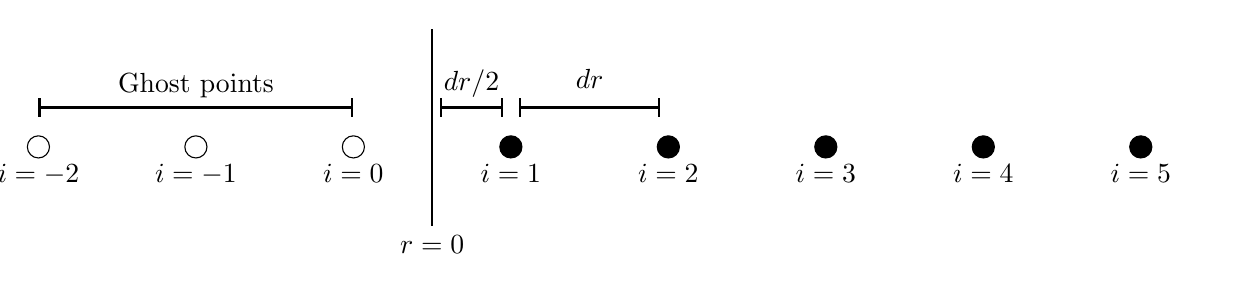
\begin{tikzpicture}
\draw[black] (-3,0) circle (4pt);
\node [below] at (-3,-0.1) {$i=-2$};
\draw[black] (-1,0) circle (4pt);
\node [below] at (-1,-0.1) {$i=-1$};
\draw[black] (1,0) circle (4pt);
\node [below] at (1,-0.1) {$i=0$};
\filldraw[black] (3,0) circle (4pt);
\node [below] at (3,-0.1) {$i=1$};
\filldraw[black] (5,0) circle (4pt);
\node [below] at (5,-0.1) {$i=2$};
\filldraw[black] (7,0) circle (4pt);
\node [below] at (7,-0.1) {$i=3$};
\filldraw[black] (9,0) circle (4pt);
\node [below] at (9,-0.1) {$i=4$};
\filldraw[black] (11,0) circle (4pt);
\node [below] at (11,-0.1) {$i=5$};
\draw[black,thick,|-|] (2.1,0.5) -- (2.9,0.5);
\node[above] at (2.5,0.5) {$dr/2$};
\draw[black,thick,|-|] (3.1,0.5) -- (4.9,0.5);
\node[above] at (4,0.62) {$dr$};
\draw[black,thick] (2,-1) -- (2,1.5);
\node [below] at (2,-1) {$r=0$};
\draw[black,thick,|-|] (-3,0.5) -- (1,0.5);
\node [above] at (-1,0.5) {Ghost points};
\end{tikzpicture}
\end{center}
\caption{Basic grid structure close to the axis of symmetry $r=0$,
  showing how the axis is staggered.  We show the case of 3 ghost
  points to the left of the origin (for fourth order spatial
  differencing).}
\label{fig:grid}
\end{figure}

The grid for the coordinate $z$, on the other hand, has two different
structures depending on whether we have or not equatorial symmetry.
If the logical parameter \texttt{eqsym} is set to \texttt{.false.}, 
that is if there is no equatorial symmetry, then the grid uses \texttt{Nz}
points along the $z$ direction starting from $-Nz/2$ to $+Nz/2$.  Notice
that of \texttt{Nz} is even then there will be no point at $z=0$ (and the
equator will be staggered9, while if \texttt{Nz} is odd there will be
a point with $z=0$.

On the other hand, if the logical parameter \texttt{eqsym} is set to
\texttt{.true.}, then the equator is always staggered and symmetry
conditions are applied in the $z$ direction in the same way as it is
done with the axis if symmetry for the coordinate $r$. Having
equatorial symmetry then reduces the use of computational by half.


\subsection{Box-in-box grid refinement}

The also code uses ``box-in-box'' type grid refinement.  That is, it
has refinement levels with higher resolution set up at the beginning
from the parameter file. The code allows one to set up to 4 different
refinement regions called ``boxes'', number 0 to 3. In each of these
refinement boxed one can also specify how many refinement levels one
needs.  Box 0 level 0 always refers to the main coarse grid.  While
Box 0 levels 1,2,3,...  refer to refinement levels on this main grid,
always with half the resolution and the same number of grid points.
So in essence, refinement levels of Box 0 always refine the region
around the origin. \\

On the other hand, boxes 1,2,3 can be placed in different parts of the
main grid. This can be useful if one need to refine a specific region
of the grid know a priori which does not correspond to the origin. \\

The total number of refinement boxes is controlled by the integer
parameter \texttt{Nb} which tells the code how many extra boxes are
required.  This parameter can take values from 0 to 3, with 0 (the
default) referring to having only the main Box 0. The number of
refinement levels on each box are given, respectively, by the
parameters \texttt{Nl0,Nl1,Nl2,Nl3}. \\

For example, if we take \texttt{Nb=0} and \texttt{Nl0=2}, meaning only
the main box with two extra refinement levels, the resulting grid
structure is shown in Figure~\ref{fig:B0L2}, where we have two extra
levels of refinement around the origin $r=z=0$ represented by the red
and green colors.

\begin{figure}[ht]
\centering 
\includegraphics[width=0.5\textwidth]{B0L2.png}
\caption{Schematic grid structure for the case with \texttt{Nb=0} and
  \texttt{Nl0=2}.}
\label{fig:B0L2}
\end{figure}

When we have more than one refinement box, \texttt{Nb=1,2,3}, the
position and size of the extra boxes is controlled by the parameters
\texttt{rbox\#,zbox\#,Nrbox\#,Nzbox\#}.  For example, if we take:
\texttt{Nb=3}, \texttt{Nl0=0}, \texttt{Nl1=Nl2=Nl3=1}, with
\texttt{(rbox1=5,zbox1=0)}, \texttt{(rbox2=0,zbox2=5)},
\texttt{(rbox3=0,zbox3=-5)}, and \texttt{(Nrbox1=Nzbox1=50)},
\texttt{(Nrbox2=Nzbox2=50)}, \texttt{(Nrbox3=Nzbox3=50)}, then we are
asking for three extra refinement boxes, centered on the points
$(5,0)$, $(0,5)$ and $(0,-5)$, which sizes $(50 \times 50)$ grid point
each.  Notice that now box 0 has no refinement levels, while boxes
1,2,3 have one refinement level each. The resulting grid structure is
represented in Figure~\ref{fig:B3L1}, with the extra refinement
boxes shown in different colors.

\begin{figure}[ht]
\centering 
\includegraphics[width=0.5\textwidth]{B3L1.png}
\caption{Schematic grid structure for the case with \texttt{Nb=3} and
  \texttt{Nl1=Nl2=Nl3=1}.}
\label{fig:B3L1}
\end{figure}

\subsection{Domain decomposition paralellization}

\vspace{3mm}


%%%%%%%%%%%%%%%%%%%%%
%%%   SPACETIME   %%%
%%%%%%%%%%%%%%%%%%%%%

\setcounter{equation}{0}
\section{Spacetime and evolution equations}

\subsection{Spacetime metric}

As already mentioned, the code uses cylindrical coordinates $(r,z)$ in
space. Notice that what the code calls $r$ here represents distance to
the symmetry axis and not distance to the origin. The distance to the
origin in the code is in fact called $rr:=(r^2 + z^2)^{1/2}$. \\

The spatial metric is written in the following way:
\begin{align}
dl^2 &= e^{4 \phi(r,z,t)} \left[ A(r,z,t) dr^2 + B(r,z,t) dz^2 
+ r^2 H(r,z,t) d\varphi^2 \right. \nonumber \\
&+ 2 \left. r \left( C(r,z,t) dr dz + r^2 C_1(r,z,t) dr d\varphi
+ r C_2(r,z,t) dz d\varphi \right) \right] \; ,
\label{eq:metric}
\end{align}
with $\phi$ the conformal factor. The powers of $r$ in some of the
terms come from the behaviour of the different metric components close
to the axis. Factorizing those powers of $r$ explicitly allows us to
make sure that the functions $(A,B,H,C,C_1,C_2)$ are well behaved at
$r=0$. Notice that the components of the extrinsic curvature $K_{ij}$
are also decomposed in a similar way (see below). \\

We also define the function $\psi = e^\phi$ and use it instead of
$\phi$ in many expressions. For the lapse function we use the array
$\alpha(r,z,t)$, while the shift in principle has three components:
$\beta^r(r,z,t)$, $\beta^z(r,z,t)$, $\beta^\varphi(r,z,t)$. \\

Notice that when there is no angular momentum the metric can be
simplified since in that case we have $\beta^\varphi=0$, and
$C_1=C_2=0$.  The code controls this using the logical parameter
\texttt{angmom}: if this parameter is true then those arrays are
turned on, while if it is false they are off.  By default the
parameter is false, so that those arrays are turned off. \\

It is also useful to define an inverse to the conformal factor as:
\begin{equation}
\chi := 1/\psi^n = \exp(-n \phi) \; ,
\end{equation}
with $n$ a power controlled by the parameter \texttt{chipower}.  For
black hole spacetimes the conformal factor $\phi$ is singular at the
black hole position, while $\chi$ remains regular, so it is best
to evolve $\chi$ instead of $\phi$. This can be controlled with the
logical parameter \texttt{chimethod} (which by default is set to
\texttt{.true.}).

\subsection{Evolution equations}

For the evolution equations, the code uses a
Baumgarte-Shapiro-Shibata-Nakamura (BSSN) formulation adapted to axial
symmetry.  The specific form of the evolution equations used here can
be found in~\cite{Alcubierre11}. \\

There are two BSSN variants or ``flavors'' controlled by the
parameter \texttt{bssnflavor}, which can take the values
\texttt{lagrangian} or \texttt{eulerian} (the
default is \texttt{bssnflavor=lagrangian}). They refer to the way in which the
shift terms are added to make determinant of the conformal metric
constant along time-lines (lagrangian), or constant along the
normal-lines (eulerian). \\

There is also a parameter that allows one to switch off the evolution
of the spacetime, which is useful in case one wants to evolve some
matter field in a fixed background spacetime. The parameter is called
\texttt{spacetime} and can have the values \texttt{dynamic} or
  \texttt{static} (default is \texttt{spacetime=dynamic}). \\

The main evolution variables (arrays) are:

\begin{list}{}{
\setlength{\leftmargin}{35mm}
\setlength{\labelsep}{10mm}
\setlength{\labelwidth}{20mm}}

\item[\texttt{alpha}] The lapse function $\alpha$.

\item[\texttt{beta\_r}] Contravariant shift component $\beta^r$.

\item[\texttt{beta\_z}] Contravariant shift component $\beta^z$.

\item[\texttt{beta\_p}] Contravariant angular shift component $\beta^\varphi$.

\item[\texttt{phi}] The conformal factor $\phi$ (see equation~\ref{eq:metric}).

\item[\texttt{psi}] The conformal factor $\psi=e^\phi$ (see
  equation~\ref{eq:metric}).

\item[\texttt{A}] Component $(r,r)$ of conformal metric $\tilde{g}_{rr}=\texttt{A}$.

\item[\texttt{B}] Component $(z,z)$ of conformal metric  $\tilde{g}_{zz}=\texttt{B}$.

\item[\texttt{H}] Component $(\varphi,\varphi)$ of conformal metric  $\tilde{g}_{\varphi \varphi}= r^2 \: \texttt{H}$.

\item[\texttt{C}] Component $(r,z)$ of conformal metric  $\tilde{g}_{rz}= r \: \texttt{C}$.

\item[\texttt{C1}] Component $(r,\varphi)$ of conformal metric $\tilde{g}_{r \varphi}= r^2 \: \texttt{C1}$.

\item[\texttt{C2}] Component $(z,\varphi)$ of conformal metric $\tilde{g}_{z \varphi}= r \: \texttt{C1}$.

\item[\texttt{trK}] Trace of the extrinsic curvature
  \mbox{$\texttt{trK} := {K^m}_m$}.

\item[\texttt{KTA}] Component $(r,r)$ of conformal trace-free extrinsic
  curvature $\tilde{K}^{TF}_{rr} = \texttt{KTA}$.

\item[\texttt{KTB}] Component $(z,z)$ of conformal trace-free extrinsic
  curvature $\tilde{K}^{TF}_{rr} = \texttt{KTA}$.

\item[\texttt{KTH}] Component $(\varphi,\varphi)$ of conformal trace-free extrinsic
  curvature $\tilde{K}^{TF}_{\varphi \varphi} = r^2 \: \texttt{KTH}$.

\item[\texttt{KTC}] Component $(r,z)$ of conformal trace-free extrinsic
  curvature $\tilde{K}^{TF}_{rz} = r \: \texttt{KTC}$.

\item[\texttt{KTC1}] Component $(r,\varphi)$ of conformal trace-free extrinsic
  curvature $\tilde{K}^{TF}_{r \varphi} = r^2 \: \texttt{KTC1}$.

\item[\texttt{KTC2}] Component $(r,\varphi)$ of conformal trace-free extrinsic
  curvature $\tilde{K}^{TF}_{z \varphi} = r \: \texttt{KTC2}$.

\item[\texttt{Delta\_r}] Contravariant component of auxiliary BSSN variable $\Delta^r$.

\item[\texttt{Delta\_z}] Contravariant component of auxiliary BSSN variable $\Delta^z$.

\item[\texttt{Delta\_p}] Contravariant component of auxiliary BSSN variable $\Delta^\varphi$.

\end{list}

Notice that, even though the auxiliary BSSN variables $\Delta^i$ are
initially defined in terms of metric derivatives, they are later
evolved independently with their own evolution equations (modified using
the momentum constraints), as required in the BSSN formulation. \\

The code also calculates a series of auxiliary geometric quantities
defined as:

\begin{list}{}{
\setlength{\leftmargin}{35mm}
\setlength{\labelsep}{10mm}
\setlength{\labelwidth}{20mm}}

\item[\texttt{psi}] The conformal factor $\texttt{psi}:=\psi=e^\phi$.
  The code also calculates $\texttt{psi2}:=\psi^2$ and
    $\texttt{psi4}:=\psi^4$.

\item[\texttt{chi}] Another form of the conformal factor
  $\texttt{chi}=\chi=1/\psi^n$.  This function is in fact evolved
  instead of $\phi$ if one sets the logical parameter
  \texttt{chimethod=.true.} (by default it is true).  This is useful
  for black hole evolutions as it improves the treatment of the
  central punctures.

\end{list}


%%%%%%%%%%%%%%%%%%%%%%%%%%
%%%   REGULARIZATION   %%%
%%%%%%%%%%%%%%%%%%%%%%%%%%


%%%%%%%%%%%%%%%%%%
%%%   MATTER   %%%
%%%%%%%%%%%%%%%%%%

\setcounter{equation}{0}
\section{Matter}
\label{sec:matter}

When we write the Einstein equations in 3+1 form, the components of
the stress-energy tensor that will be important are the energy density,
momentum density and spatial stress tensor as measured by the
so-called Eulerian observers, {\em i.e.} those that move along
the normal direction to the spatial hypersurfaces:
\begin{eqnarray}
\rho &=& n^\mu n^\nu T_{\mu \nu} \; , \\
J_i &=& - n^\mu P_i^\nu T_{\mu \nu} \; , \\
S_{ij} &=& P_i^\mu P_i^\nu T_{\mu \nu} \; ,
\end{eqnarray}
with $n^\mu$ the unit normal vector to the spatial hypersurfaces of
constant coordinate time, and $P^\mu_\nu$ the projector operator onto
these hypersurfaces. \\

The code defines as 2D arrays the energy density \texttt{rho}, the
three components of the momentum density (index up) \texttt{J\_r},
\texttt{J\_z}, \texttt{J\_p} (where the index ``p'' stands for the
$\varphi$ component), and the six components of the spatial stress
tensor which is decomposed in the same way as the metric and
extrinsic curvature: \texttt{S\_A,S\_B,S\_H,S\_C,S\_C1,S\_C2}.
Additionally, the trace of the spatial stress tensor is also defined
as \texttt{trS}.  In the code these quantities are defined even for
vacuum (they are set to zero), since they are required both in the
evolution equations and for the calculation of the constraints. \\

The type of matter used by the code is controlled by the
character-type parameter \texttt{mattertype}.  At the moment it allows
the following values:

\begin{list}{}{
\setlength{\leftmargin}{35mm}
\setlength{\labelsep}{10mm}
\setlength{\labelwidth}{30mm}}

\item[\texttt{vacuum}] There is no matter (this is the default).

\item[\texttt{scalar}] Real scalar field.  The scalar field is assumed
  to have a potential whose form is controlled by the parameter
  \texttt{scalarpotential}, which can take the values
  (\texttt{none,phi2,phi4}), corresponding to a free scalar field
  (\texttt{none}), a massive scalar field with a
  potential of the form $V=m^2 \Phi^2/2$
  (\texttt{phi2}), where the mass $m$ is give by the
  parameter \texttt{scalar\_mass}, or a potential of the form
  $V=m^2 \Phi^2/2 + \lambda \Phi^4 / 4$
  (\texttt{phi4}), with the coefficient of the
  self-interaction term given by the parameter
  \texttt{scalar\_lambda}.

\item[\texttt{complex}] Complex scalar field.  The complex scalar
  field is assumed to have a potential whose form is controlled by the
  parameter \texttt{complexpotential}, which can take the values
  (\texttt{none,phi2,phi4}), corresponding to a free scalar field
  (\texttt{none}), a massive scalar field with a potential of the form
  $V=m^2 |\Phi|^2/2$ (\texttt{phi2}), where the mass $m$ is give by
  the parameter \texttt{complex\_mass}, or a potential of the form
  $V(\phi)=m^2 |\Phi|^2/2 + \lambda |\Phi|^4 / 4$ (\texttt{phi4}),
  with the coefficient of the self-interaction term given by the
  parameter \texttt{complex\_lambda}.

\end{list}

Any new type of matter model should be added to the list of allowed
values for this parameter in the file \texttt{param.f90}. Notice that
the code allows one to have several different types of matter at the
same time, the corresponding stress-energy tensors are just added
together. For example, if you want to have a real scalar field and a
complex scalar field evolving together you can add the following line
to the parameter file: \\

\texttt{mattertype = scalar,complex} \\


%%%%%%%%%%%%%%%%%%%%%%%
%%%   CONSTRAINTS   %%%
%%%%%%%%%%%%%%%%%%%%%%%

\setcounter{equation}{0}
\section{Constraints}
\label{sec:constraints}

\subsection{Hamiltonian and momentum constraints}

When required for output, the code calculates the Hamiltonian and the
three components of the momentum constraints (index up) and saves them
in the arrays \texttt{ham} and \texttt{mom\_r}, \texttt{mom\_z},
\texttt{mom\_p} (read the comments in the routine
\texttt{src/geometry/constraints.f90} to see how they are
calculated). \\

Notice that for an exact solution both these constraints should be
zero, so monitoring their behaviour, and particularly how they
approach zero as we increase the resolution, gives us information
about the accuracy of the code. \\

\subsection{BSSN extra constraints}

The BSSN formalism requires the introduction of the auxiliary variables
$\Delta^i$ defined in terms of derivatives of the conformal metric
components (see~\cite{Alcubierre11}).  These are then promoted
to independent variables, and their evolution equations are modified
using the momentum constraints. \\

We therefore end up with a new constraints related to the definition
of the $\Delta^i$ that are calculated for output in the arrays
\texttt{CDelta\_r}, \texttt{CDelta\_z} and \texttt{CDelta\_p} (read the
comments in the routine \texttt{src/geometry/constraints.f90} to see
how they are calculated).

\vspace{3mm}


%%%%%%%%%%%%%%%%%%%%%%%%%%%%%%
%%%   SLICING CONDITIONS   %%%
%%%%%%%%%%%%%%%%%%%%%%%%%%%%%%

\setcounter{equation}{0}
\section{Slicing conditions}
\label{sec:slicing}

The slicing condition is controlled by the parameter \texttt{slicing},
which at the moment can take one of the following values (default is
\texttt{slicing=harmonic}):

\begin{list}{}{
\setlength{\leftmargin}{35mm}
\setlength{\labelsep}{10mm}
\setlength{\labelwidth}{20mm}}

\item[\texttt{static}] The lapse remains static at its initial value and does not evolve.

\item[\texttt{harmonic}] This is a harmonic-type slicing condition of the form:
\begin{equation}
\partial_t \alpha = - \alpha^2 f \: {\rm tr} K + \beta^m \partial_m \alpha \; ,
\end{equation}
where $f$ is a real positive number controlled by the parameter
\texttt{gauge\_f} (default is \texttt{gauge\_f=1}). True harmonic
slicing really corresponds to \texttt{gauge\_f=1}, but here we allow
any positive real number.  This is a hyperbolic slicing condition
corresponding to a speed of propagation of the gauge given by
$\sqrt{f}$.

\item[\texttt{1+log}] This is a slicing condition of the 1+log family,
  which is very similar to the harmonic family above:
\begin{equation}
\partial_t \alpha = - \alpha f \: {\rm tr} K + \beta^m \partial_m \alpha \; ,
\end{equation}
where again $f$ is a positive real number controlled by the same
parameter \texttt{gauge\_f}.  Standard 1+log slicing corresponds to 
\texttt{gauge\_f=2} (though as mentioned above the default value is 1).

\item[\texttt{shockavoid}] This corresponds to the family of shock
  avoiding slicing conditions, which is similar to the 1+log
  condition above but with $f(\alpha)$ a function given by (see
    comments in file \texttt{src/geometry/auxiliary\_geometry.f90}):
\begin{equation}
f(\alpha) = 1 + k/\alpha^2 \; .
\end{equation}
The code takes $k=\texttt{gauge\_f}-1$.

\item[\texttt{maximal}] This is maximal slicing which corresponds to
  the condition that the trace of the extrinsic curvature remains
  equal to zero during evolution (which guarantees that the spatial
  volume elements remain constant), and which implies that the lapse
  must satisfy the following elliptic equation:
\begin{equation}
\nabla^2 \alpha = \alpha K_{ij} K^{ij} + 4 \pi \alpha  \left( \rho + {\rm tr} S \right) \; .
\end{equation}

\end{list}

\vspace{3mm}

Notice that the choices \texttt{harmonic}, \texttt{1+log} and
\texttt{shockavoid} are special cases of the Bona-Masso family of
slicing conditions that has the general form:
\begin{equation}
\partial_t \alpha = - \alpha^2 f(\alpha) {\rm trK} + \beta^r \partial_r \alpha\; .
\end{equation}
with $f(\alpha)$ an arbitrary (positive) function of the lapse.
 
\vspace{5mm}

The initial value of the lapse can also be controlled by the parameter
\texttt{ilapse} which can take the values (default
\texttt{ilapse=none}):

\begin{list}{}{
\setlength{\leftmargin}{35mm}
\setlength{\labelsep}{10mm}
\setlength{\labelwidth}{20mm}}

\item[\texttt{none}] The initial lapse it first set to 1, but can
  later be modified by initial data routines and will not be touched
  after this.

\item[\texttt{one}] The initial lapse is set to 1 again AFTER all
  initial data routines have been called.

\item[\texttt{isotropic}] The initial lapse is set to the
  corresponding isotropic lapse for a single static black hole (useful
  for testing).

\item[\texttt{psiminus2}] The initial lapse is set to
  $\alpha=1/\psi^2$ after all initial data routines have been called,
  with $\psi$ the conformal factor. This is useful for black hole
  evolutions where $\psi$ becomes infinite at the origin, and results
  in a ```pre-collapsed'' initial lapse that is already zero and
  smooth at $r=0$.

\item[\texttt{psiminus4}] Similar to the case above, but sets the
  initial lapse to $\alpha=1/\psi^4$.

\item[\texttt{maximal}] The maximal slicing condition is solved for
  the initial lapse, but the lapse can later be evolved using a
  different condition.

\end{list}

\vspace{5mm}

There is also the possibility of adding a Gaussian to the initial
value of the lapse. This is useful for perturbing the initial data and
causing interesting gauge dynamics.  This is controlled by the
parameters:

\begin{list}{}{
\setlength{\leftmargin}{35mm}
\setlength{\labelsep}{10mm}
\setlength{\labelwidth}{20mm}}

\item[\texttt{lapsegauss}] Logical parameter that if set to
  \texttt{.true.} adds a Gaussian to the initial lapse (default is
  \texttt{.false.}).

\item[\texttt{lapse\_a0}] Amplitude of Gaussian.

\item[\texttt{lapse\_r0}] Center of Gaussian in $r$ direction.

\item[\texttt{lapse\_sr0}] Width of Gaussian in $r$ direction.

\item[\texttt{lapse\_z0}] Center of Gaussian in $z$ direction.

\item[\texttt{lapse\_sz0}] Width of Gaussian in $z$ direction.

\end{list}

\vspace{3mm}


%%%%%%%%%%%%%%%%%%%%%%%%%%%%
%%%   SHIFT CONDITIONS   %%%
%%%%%%%%%%%%%%%%%%%%%%%%%%%%

\setcounter{equation}{0}
\section{Shift conditions}
\label{sec:shift}

The shift condition is controlled by the parameter \texttt{shift},
which at the moment can take one of the following values (default is
\texttt{shift=none}):

\begin{list}{}{
\setlength{\leftmargin}{45mm}
\setlength{\labelsep}{10mm}
\setlength{\labelwidth}{30mm}}

\item[\texttt{none}] There is no shift, and all shift terms in the
  evolution equations are ignored.  This is the default.

\item[\texttt{zero}] The shift is set to zero, but all the shift terms
  in the evolution equations are calculated.  This is useful for
  testing.

\item[\texttt{static}] The shift is non-zero but it does not evolve in
  time. Again, useful for testing.

\item[\texttt{Gammadriver1}] Parabolic Gamma-driver shift.  The shift
  condition is given by:
\begin{equation}
\partial_t \beta^i = \xi \partial_t \Delta^i \; .
\end{equation}

\item[\texttt{Gammadriver2}] Standard second order hyperbolic
  Gamma-driver shift.  The shift condition is given by:
\begin{equation}
\partial^2_t \beta^i = \xi \partial_t \Delta^i - \eta \partial_t \beta^i \; .
\end{equation}
In the code this is written in second order form as:
\begin{eqnarray}
\partial_t \beta^i &=& {\cal B}^i \; , \\
\partial_t {\cal B}^i &=& \xi \partial_t \Delta^i - \eta {\cal B}^i \; .
\end{eqnarray}
This is in fact the standard Gamma-driver used in most BSSN codes.
Notice that in the code the components of ${\cal B}^i$ are in fact
called (\texttt{dtbeta\_r}, \texttt{dtbeta\_z}, \texttt{dtbeta\_p}).

\end{list}

\vspace{3mm}

The Gamma-driver shift conditions above relate the evolution of the
shift to that of the BSSN auxiliary variables $\Delta^i$. The values
of the coefficients $\xi$ and $\eta$ are controlled with the real
parameters \texttt{drivercsi} and \texttt{drivereta}.  There is also
the logical parameter \texttt{driveradv} which if set to
\texttt{.true.}  modifies the Gamma driver conditions by adding
advection terms on the shift (by default it is \texttt{.false.}). \\

Just as in the case of the lapse, there is the possibility of adding a
Gaussian to the initial value of the shift. This is useful for
perturbing the initial data and causing interesting gauge dynamics.



%%%%%%%%%%%%%%%%%%%%%%%%%%%%%%%
%%%   BOUNDARY CONDITIONS   %%%
%%%%%%%%%%%%%%%%%%%%%%%%%%%%%%%

\setcounter{equation}{0}
\section{Boundary conditions}
\label{sec:boundary}

The outer boundary conditions for the evolution are controlled by the
character-type parameter \texttt{boundary}, which at the moment can
take one of the following values (the default is \texttt{flat}):

\begin{list}{}{
\setlength{\leftmargin}{35mm}
\setlength{\labelsep}{10mm}
\setlength{\labelwidth}{25mm}}

\item[\texttt{none}] No boundary condition is applied.  The sources are
  applied all the way to the boundary using one-sided differences.

\item[\texttt{static}] The sources are set to zero at the boundary.
  This is done only for evolving arrays that are not declared with the
  keyword \texttt{NOBOUND}.

\item[\texttt{flat}] The sources at the boundary are copied from their
  value one grid point in. This is done only for evolving arrays that
  are not declared with the keyword \texttt{NOBOUND}.

\item[\texttt{radiative}] Outgoing-wave boundary condition. This is
  somewhat more involved as it uses some information from eigenfields
  and eigenspeeds, and works quite well in practice.

\end{list}

\vspace{3mm}

Notice that all the boundary conditions are always applied at the
level of the source terms, and are applied only for some of the
evolving arrays and not all of them.  In general, evolving arrays that
are declared with the keyword \texttt{NOBOUND} have no need for a
boundary condition since their source terms can be calculated all the
way to the boundary. \\

Static and flat boundary conditions are applied in the automatically
generated file \linebreak \texttt{src/auto/simpleboundary.f90}.  The
radiative boundary conditions are explained with more detail below.

\subsection{Radiative boundaries}


%%%%%%%%%%%%%%%%%%%%%%%%
%%%   INITIAL DATA   %%%
%%%%%%%%%%%%%%%%%%%%%%%%

\setcounter{equation}{0}
\section{Initial data}
\label{sec:initial}

The type of initial data is controlled by the character-type parameter
\texttt{idata}.  If you add a new type of initial data it should be
appended to the list of allowed values for this parameter in the file
\texttt{src/base/param.f90}.  You should also add a corresponding call to your
initial data routine in the file \texttt{src/base/initial.f90}. \\

Simple types of vacuum initial data already there are:

\begin{list}{}{
\setlength{\leftmargin}{55mm}
\setlength{\labelsep}{10mm}
\setlength{\labelwidth}{50mm}}

\item[\texttt{idata=minkowski}] The initial metric is simply set to
  Minkowski and the extrinsic curvature is set to zero.  Notice that
  one can still have non-trivial gauge evolution if one adds a
  Gaussian perturbation to the initial lapse (see
  Section~\ref{sec:slicing}).

\item[\texttt{idata=schwarzschild}] The initial metric is set to that
  corresponding to a Schwarzschild black hole in isotropic coordinates
  centered at the origin. The mass of the black hole controlled by the
  parameter \texttt{BH1mass} (default is 1).  The initial extrinsic
  curvature is set to zero.

\item[\texttt{idata=BrillLindquist}] This is initial data for two black
  holes in isotropic (conformally flat) coordinates. The masses of the
  two black holes are controlled by the parameters \texttt{BH1mass}
  and \texttt{BH2mass}, and their position on the $z$ axis is
  controlled by the parameters \texttt{BH1Z} and \texttt{BH2Z}.

\end{list}


%%%%%%%%%%%%%%%%%%%%
%%%   HORIZONS   %%%
%%%%%%%%%%%%%%%%%%%%

\setcounter{equation}{0}
\section{Horizon finder}
\label{sec:horizon}


%%%%%%%%%%%%%%%%%%%%%%%%%%%
%%%   WAVE EXTRACTION   %%%
%%%%%%%%%%%%%%%%%%%%%%%%%%%

\setcounter{equation}{0}
\section{Gravitational wave extraction}
\label{sec:waves}


%%%%%%%%%%%%%%%%%%%%%%%%%%%%%
%%%   NUMERICAL METHODS   %%%
%%%%%%%%%%%%%%%%%%%%%%%%%%%%%

\setcounter{equation}{0}
\section{Numerical methods}
\label{sec:numerics}

\subsection{Time integration}

For the time integration the code uses a method of lines, where the
time integration and spatial differentiation are considered
independent of each other. \\

For the evolution of the field variables we can use one of two
methods:

\begin{enumerate}

\item Standard fourth order Runge-Kutta.

\item 3-step iterative Crank-Nicholson scheme (ICN).  The ICN scheme for
N iterations is defined as follows (with $S(f)$ the source term of the
evolution equation):
\begin{eqnarray}
f_0  &=&  f(t) \; , \\
f_{i+1} &=&  f_0 + dt/2 \; S(f_i)  \qquad \textrm{i from 1 to N-1} \; , \\
f_N &=&  f_0 + dt \; S(f_{N-1}) \; , \\
f_t+dt &=& f_N
\end{eqnarray}

That is, we do $N-1$ half steps starting always from $f(t)$ but
evaluating the source term using the results from the previous step.
Finally, we do one last full step.  Doing only 2 ($N=2$) steps is
enough for second order accuracy, but we need to do at least 3 ($N=3$)
for stability.  ICN is a rather robust method that can be applied to
non-linear systems of equations, but it is somewhat dissipative.

\end{enumerate}

The choice of the integration method is done through the parameter
\texttt{integrator} which can take the values \{\texttt{rk4,icn}\}. \\

\subsection{Spatial differencing}

For spatial differentiation we can use either second or fourth order
differencing (I have also added sixth and eight order, but this is
usually not needed as the time integration is at most fourth order).
Close to the outer boundaries we in fact reduce the differencing
always to second order.  The choice of the differencing order is
controlled by the parameter \texttt{order} which can take the values
\{\texttt{two,four}\}. \\

\subsection{Dissipation}

The code uses Kreiss-Oliger type dissipation to improve stability.
Often one can turn this off and things will still work, but is seems
to be important for scalar field evolutions and also to keep a black
hole spacetimes stable for a long time. The dissipation of the
geometric variables is controlled by the parameter \texttt{geodiss},
and the dissipation for the scalar field (both real and complex) is
controlled by the parameter \texttt{scalardiss}. Both are set by
default to a value of 0.01.


%%%%%%%%%%%%%%%%%%%%%%%%%%%%
%%%   ELLIPTIC SOLVERS   %%%
%%%%%%%%%%%%%%%%%%%%%%%%%%%%

\setcounter{equation}{0}
\section{Elliptic solvers}
\label{sec:elliptic}

For solving initial data, as well as some gauge conditions such as
maximal slicing, we need to have elliptic equation solvers in the code
At the moment there are only two very simple (and slow) elliptic
solvers (and they have not been very heavily tested). \\

The choice of elliptic solver is controlled by the parameter \texttt{ELL\_solver}
which can take the following values:

\begin{list}{}{
\setlength{\leftmargin}{55mm}
\setlength{\labelsep}{10mm}
\setlength{\labelwidth}{50mm}}

\item[\texttt{ELL\_solver=none}] No elliptic solver is active.

\item[\texttt{ELL\_solver=wave}] Solver based on turning the
elliptic equation into a wave-type hyperbolic equation and
evolving this in fictitious time until we reach a steady state.

\item[\texttt{ELL\_solver=sor}] Simple elliptic SOR solver. 

\end{list}


%%%%%%%%%%%%%%%%%%%%%%%%%%%%%%
%%%   LIST OF PARAMETERS   %%%
%%%%%%%%%%%%%%%%%%%%%%%%%%%%%%

\section{List of main code parameters}
\label{sec:parameters}

Here is a list of the main code parameters with their default values
and ranges when applicable.  For a list of all declared parameters see
the file \texttt{src/base/param.f90}.  But do notice that some of the
``parameters'' declared in \texttt{param.f90} should not be fixed in
the parameter file since they are in fact defined at run time. \\

There are many more parameters that are not mentioned here,
particularly related to matter models or initial data routines.  Have
a look at the file \texttt{src/base/param.f90} where they are defined,
they are usually explained in the comments).

\begin{itemize}

\item Grid parameters:

\begin{list}{}{
\setlength{\leftmargin}{60mm}
\setlength{\labelsep}{10mm}
\setlength{\labelwidth}{50mm}}

\item[\texttt{dr0 (real)}] Spatial interval along $r$ direction for
  base (coarsest) grid (default 1.0).

\item[\texttt{dz0 (real)}] Spatial interval along $z$ direction for
  base (coarsest) grid (default 1.0).

\item[\texttt{Nrtotal (integer)}] Total number of grid points along
  $r$ direction for base grid (default 10).

\item[\texttt{Nztotal (integer)}] Total number of grid points along
  $r$ direction for base grid (default 10).

\item[\texttt{Nb (integer)}] Number of refinement boxes other than the
  main one, as much as 3 (default 0). Notice that this does NOT mean
  the number of refinement levels, but rather the number of different
  regions to be refined.

\item[\texttt{Nl0 (integer)}] Number of extra refinement levels on main
  box centered on the origin (default 0).

\item[\texttt{Nl* (integer)}] Number of extra refinement levels on
  refinement box *, with *$=(1,2,3)$ (default 0).

\item[\texttt{eqsym} (logical)] Do we have equatorial symmetry?
  (default \texttt{.false.}).

\item[\texttt{ghost (integer)}] Number of ghost zones (default 0).
  Should NOT be fixed in the parameter file.

\item[\texttt{interporder (character)}] Order of interpolation
  (default ``bicubic'').  Don't change this unless you know what you
  are doing!

\item[\texttt{boundtype (character)}] Type of outer boundary condition.
  Can take the following values: \texttt{none}, \texttt{static},
  \texttt{flat}, \texttt{radiative} (default \texttt{radiative}).

\end{list}

\item Time stepping parameters:

\begin{list}{}{
\setlength{\leftmargin}{60mm}
\setlength{\labelsep}{10mm}
\setlength{\labelwidth}{50mm}}

\item[\texttt{dtfac (real)}] Currants parameter (default 0.5).

\item[\texttt{dt0 (real)}] Time step for base (coarsest) grid
  (default 0.0).  This should NOT be set in the parameter file, as it
  is calculated at run time based on the value of \texttt{dt0} and
  \texttt{dtfac}: \texttt{dt0 = dtfac*min(dr0,dz0)}. 

\item[\texttt{adjuststep (logical)}] Dynamically adjust the time step in order
to satisfy the Courant stability condition (default .false.).

\item[\texttt{Nt (integer)}] Total number of time steps (default 10).

\end{list}

\item Output parameters:

\begin{list}{}{
\setlength{\leftmargin}{60mm}
\setlength{\labelsep}{10mm}
\setlength{\labelwidth}{50mm}}

\item[\texttt{directory (character)}]  Name of output directory (default \texttt{output}).

\item[\texttt{Ninfo (integer)}] Frequency of output to screen (default 1).

\item[\texttt{Noutput0D (integer)}] Frequency of 0D output (default 1).

\item[\texttt{Noutput1D (integer)}] Frequency of 1D output (default 1).

\item[\texttt{Noutput2D (integer)}] Frequency of 2D output (default 1).

\item[\texttt{outvars0D (character)}] Comma separated lists of
variables that need 0D output (default \texttt{alpha}).

\item[\texttt{outvars1D (character)}] Comma separated lists of
variables that need 1D output (default \texttt{alpha}).

\item[\texttt{outvars2D (character)}] Comma separated lists of
variables that need 2D output (default \texttt{alpha}).

\item[\texttt{commentype (character)}] Type of comment lines used on the
output files \linebreak (range = \{\texttt{xgraph}, \texttt{gnuplot}\}, default
\texttt{xgraph}).

\item[\texttt{outparallel (character)}] Type of parallel output (range
  = \{\texttt{singlefile}, \texttt{fileperproc}\}, default
  \texttt{fileperproc}).

\end{list}

\item Evolution parameters:

\begin{list}{}{
\setlength{\leftmargin}{60mm}
\setlength{\labelsep}{10mm}
\setlength{\labelwidth}{50mm}}

\item[\texttt{spacetime (character)}] Can take the values
  \texttt{dynamic} or \texttt{background} to choose if we want a
  dynamic spacetime (evolve the Einstein field equations) or a static
  background spacetime (default \texttt{dynamic}).

\item[\texttt{formulation (character)}] Defines the formulation of the
  3+1 equations to use, and can take the values \texttt{bssn} or
  \texttt{z4c} (default \texttt{bssn}).

\item[\texttt{bssnflavor (character)}] Controls the evolution of the
  volume element in BSSN, and can take the values \texttt{lagrangian}
  or \texttt{eulerian} (default \texttt{lagrangian}).

\item[\texttt{integrator (character)}] Method for time
  integration. Can take the values \texttt{icn} for 3-step
  iterative Crank-Nicholson, or \texttt{rk4} for fourth order
  Runge-Kutta (default \texttt{icn}).

\item[\texttt{order (character)}] Order of spatial
  finite-differencing.  Can take the values \texttt{two} o
  \texttt{four} (default \texttt{two}).

\item[\texttt{chimethod (logical)}] If true evolve $\chi = \exp(-n
  \phi)$ instead of $\phi$.  This is useful for black hole evolutions
  (default \texttt{.false.}).

\item[\texttt{chipower (integer)}] Value of $n$ in the definition
  $\chi = \exp(-n \phi)$ (default \texttt{2}).

\item[\texttt{eta (real)}] Parameter that controls the multiple of the
  momentum constraints that is added to the evolution equation for the
  $\Delta^i$ in the BSSN formulation (default \texttt{2.0}).

\item[\texttt{angmom (logical)}] Do we turn on angular momentum terms
  (default \texttt{.false.}).

\item[\texttt{idata (character)}] Type of initial data (default ``minkowski'').

\item[\texttt{slicing (character)}] Type of slicing condition (default
  ``harmonic'').

\item[\texttt{geodiss (real)}] Kreiss-Oliger dissipation coefficient
  for geometric variables.

\end{list}

\end{itemize}


%%%%%%%%%%%%%%%%%%%%%%%%%%%%
%%%   EDITING THE CODE   %%%
%%%%%%%%%%%%%%%%%%%%%%%%%%%%

\section{Editing the code}
\label{sec:editing}

If you are planning to edit the code and add your own new parameters,
arrays or routines, here are some details you should know. \\


\subsection{Adding parameters}

All parameters for the code should be declared in the file
\texttt{src/base/param.f90}, using a very specific format: \\

\texttt{type :: name = value} \\

Here \texttt{type} can be any of the standard \texttt{FORTRAN}
variable types (\texttt{logical}, \texttt{integer}, \texttt{real},
\texttt{character}), \texttt{name} is the name of the parameter, and
\texttt{value} is a default initial value that makes some sense for
the code.  Only one parameter can be declared per line, since this
file will be read at compilation time by a perl script that expects
that structure. \\

The following variations are permitted:  Character-type parameters
that are allowed to receive multiple values at the same time
(separated by commas) should be declared as: \\

\texttt{character :: name = value     ! multiple} \\

Also, a range can be defined for character-type parameters as: \\

\texttt{character :: name = value     ! range = (value1,value2,...,valuen)} \\

The range is not compulsory.  If it is not there, any value
is allowed (for example, directory names). \\

REMEMBER: All parameters must have a default value, as otherwise the
code will not compile.  The initial value should basically correspond
to the code NOT doing anything weird.  That is, initialize to
Minkowski, static slicing, no shift, vacuum, and all special features
turned off. \\


\subsection{Adding arrays}

Since this is a 2D code, it works with a series of 2D arrays that have
all the dynamical and analysis variables. All arrays must be declared
in the file \texttt{src/base/arrays.config}, using a very specific format. \\


%%%%%%%%%%%%%%%%%%%%%%
%%%   OLLINGRAPH   %%%
%%%%%%%%%%%%%%%%%%%%%%

\section{Ollingraph}
\label{sec:ollingraph}

The code includes a simple 1D visualization package called
``ollingraph''.  It is written in Python and uses Matplotlib to plot
simple line plots and animations.  At the moment it should work fine
under python 3.11. It is supposed to have similar functionality to
the old xgraph and ygraph packages, and expects the data files in the
same format (see below). \\

The plots are quite simple, and meant for quick/dirty interactive
visualization.  These plots are not supposed to be used for figures
intended for publication (use gnuplot or something similar for
that). To use the package type: \\

\texttt{ollingraph  file1 file2 ... filen} \\

When plotting several data files at once, they are all assumed to be
of the same type.  One can also add a custom name for the plot using
the option --title: \\

\texttt{ollingraph --title="Plot name" file1 file2 ... filen} \\

If this option is not there the plot is just named after the name of
the data file being plotted, assuming there is only one, or just says
``Multiple data files'' if there is more than one file. \\

Before using it make sure that \texttt{ollingraph} has execution
permission: \\

\texttt{chmod +x ollingraph} \\

There is also a package for simple plots of 2D arrays called
\texttt{ollingraph2D}. It is called in a similar way:

\texttt{ollingraph2D  file} \\

But in this case the file to be plotted must have extension
\texttt{.2D}.

\vspace{5mm}

The data files are expected to have the following format:

\begin{itemize}

\item 0D files (those ending in .tl):

\begin{enumerate}

\item One comment line starting with \texttt{\#} or \texttt{"} with
  the file name (this line could be missing and it should still work).

\item A series of lines with the data points, with the x and y values
  separated by blank spaces.

\end{enumerate}

\item 1D evolution-type files (those ending in .rl):

\begin{enumerate}

\item Each time step begins with a comment line starting with
  \texttt{\#} or \texttt{"} that contains the time in the format: \\

\texttt{\#Time = (real number)} \\

\item A series of lines with two columns, with the x and y values
  separated by blank spaces.

\item One or more blank lines to separate the next time step.

\end{enumerate}

\item 2D evolution-type files (those ending in .2D):

\item Each time step begins with a comment line starting with
  \texttt{\#} or \texttt{"} that contains the time in the format: \\

\texttt{\#Time = (real number)} \\

\item A series of lines with three columns, with values separated by
  blank spaces, corresponding to the coordinates $(r,z)$ and the value
  of the corresponding variable. The values are stored by first
  looping over the $r$ coordinate with fixed value of $z$, and
  separating by blank spaces for differen values of $z$.

\end{itemize}


%%%%%%%%%%%%%%%%%%%%%%
%%%   REFERENCES   %%%
%%%%%%%%%%%%%%%%%%%%%%

\begin{thebibliography}{99}

\bibitem{Alcubierre08} ``Regularization of spherical and axisymmetric
  evolution codes in numerical relativity'', M. Ruiz, M. Alcubierre,
  D. Nuñez, Gen.Rel.Grav. {\bf 40}, 159-182 (2008); arXiv:0706.0923
  [gr-qc].

\bibitem{Alcubierre11} ``Formulations of the 3+1 evolution equations
  in curvilinear coordinates'', M.~Alcubierre and M.~D.~Mendez,
  Gen.Rel.Grav. {\bf 43}, 2769 (2011); arXiv:1010.4013 [gr-qc].

\end{thebibliography}


%%%%%%%%%%%%%%%
%%%   END   %%%
%%%%%%%%%%%%%%%

\end{document}

